\section{Experiments}
\label{sec:experiments}

We use three controlled experiments to test the mechanism suggested by the
theory. The first two are small finite-state examples that isolate norm
mismatch. The third is a continuous linear-Gaussian benchmark designed to test
whether occupancy weighting improves the parts of the fitted \(Q\)-function that
matter for policy evaluation.

\textbf{Toy norm-mismatch checks.}
We first revisit Baird's seven-state hub-and-spokes example
\citep{baird1995residual}. The target policy always takes the solid action,
which moves to the hub, while the behavior policy takes that action with
probability \(\kappa\). Smaller \(\kappa\) weakens stationary overlap. With the
standard linear feature map and exact stationary ratios, unweighted FQE slows
markedly as overlap decreases, while stationary-weighted FQE keeps nearly the
same geometric decay (Figure~\ref{fig:experiments-composite}A). We then use
100-state sparse Garnet MDPs with a low-dimensional linear class that contains
\(Q^\pi\) but is not Bellman complete. Under reset sampling and large discount,
standard FQE undergoes a sharp divergence transition, whereas exact
stationary-weighted FQE remains stable (Figure~\ref{fig:experiments-composite}B).
These examples are intentionally diagnostic: the ratios are known, so the
experiment tests the regression geometry rather than density-ratio estimation.

\textbf{Controlled continuous benchmark.}
Our main experiment uses a two-dimensional linear-Gaussian controlled Markov
process,
\[
S_{t+1}=B S_t + C A_t+\epsilon_t,\qquad
r(s,a)=-\|s-s^\star\|^2-\lambda a^2 ,
\]
with Gaussian linear behavior and target policies. The target gain is fixed and
the behavior gain is shifted away from it, producing low, moderate, and severe
behavior-target mismatch. We compute \(Q^\pi,V^\pi\), and the policy value
analytically, and evaluate errors under the target reference distribution used
by the weights. FQE uses value discount \(\gamma=0.95\). The weighting target is
varied separately: \(\gamma_{\rm ratio}\in\{0.95,0.99,1\}\), where
\(\gamma_{\rm ratio}=1\) is the stationary state-action ratio and the smaller
values are discounted-occupancy ratios that regularize the stationary limit.

The main setting uses a misspecified affine \(Q\)-class. We compare standard
FQE, oracle clipped weighting, estimated clipped linear ratios, and a
torch-based neural/RKHS ratio estimator; all hyperparameters are fixed across
shifts. Figure~\ref{fig:experiments-composite}C shows the main effect. At low
shift, weighting is essentially unnecessary. At moderate shift, standard FQE has
large target-reference \(Q\) error, while all weighted fits reduce that error
substantially. At severe shift, weighting still improves target-reference error,
but the diagnostics in Figure~\ref{fig:experiments-composite}D show the price:
raw oracle weights have small effective sample size and large upper quantiles.
This is the expected poor-overlap regime, not a hidden tuning failure.

\begin{figure}[t]
    \centering
    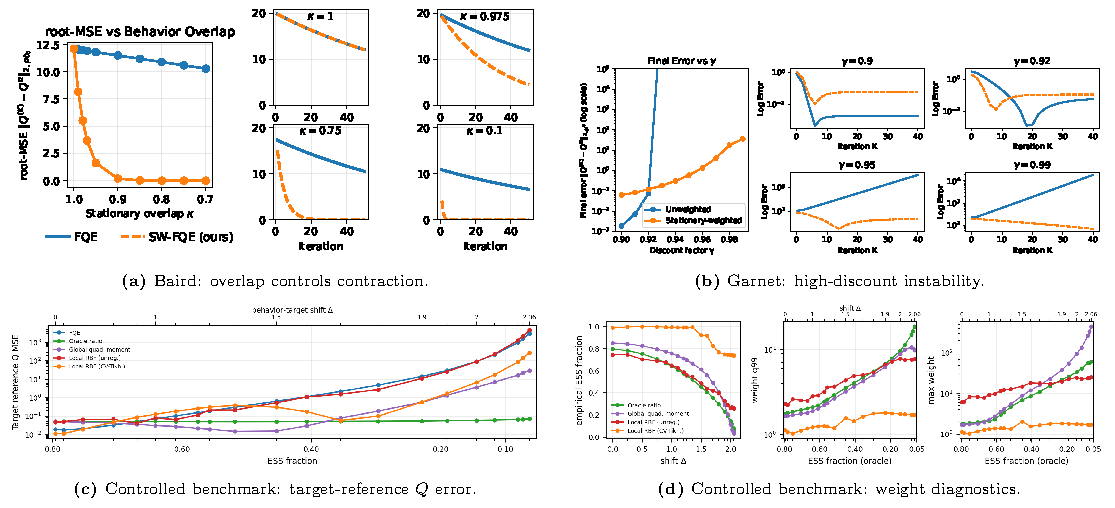
\includegraphics[width=\linewidth]{figures/experiments_composite.pdf}
    \caption{\textbf{A--B:} finite-state norm-mismatch checks. Stationary
    weighting restores fast decay in Baird's example and prevents the high
    discount divergence seen in Garnet MDPs. \textbf{C--D:} continuous
    linear-Gaussian benchmark. Weighting improves target-reference \(Q\) error
    under moderate misspecification, while ESS and upper weight quantiles expose
    the severe-shift overlap problem.}
    \label{fig:experiments-composite}
\end{figure}

Table~\ref{tab:controlled-benchmark} gives the corresponding 100-seed summary
for \(\gamma_{\rm ratio}=0.95\). The pattern is the one predicted by the
projection-norm view: weighting helps where the function class must choose
which state-action regions to approximate well. With a neural FQE class the
same effect is weaker but still visible for \(\gamma_{\rm ratio}=0.99\); the
network already reduces much of the approximation mismatch, so noisy weights no
longer help uniformly. Full settings and diagnostics are in
Appendix~\ref{sec::appendix}.
